Esta librería realiza la presentación de documentos NCL. Esto es iniciar, pausar o detener la aplicación ginga definida en el documento NCL.
Es la encargada de iniciar el parsing del documento, indicándole el nombre del archivo NCL al módulo \emph{ncl30-converter}.
Interactúa con los módulos \emph{ncl30} y \emph{gingaplayer} al leer las propiedades del modelo NCL y luego aplicarlas a los players.\\
En esta librería se definen también, clases para el manejo de los eventos descriptos en la especificación \emph{Ginga}, entre los cuales están:
\begin{itemize}[noitemsep,nolistsep]
\item Eventos de presentación.
\item Eventos de selección.
\item Eventos de seteo de propiedades.
\end{itemize}

\begin{figure}[h!]
	\centering
	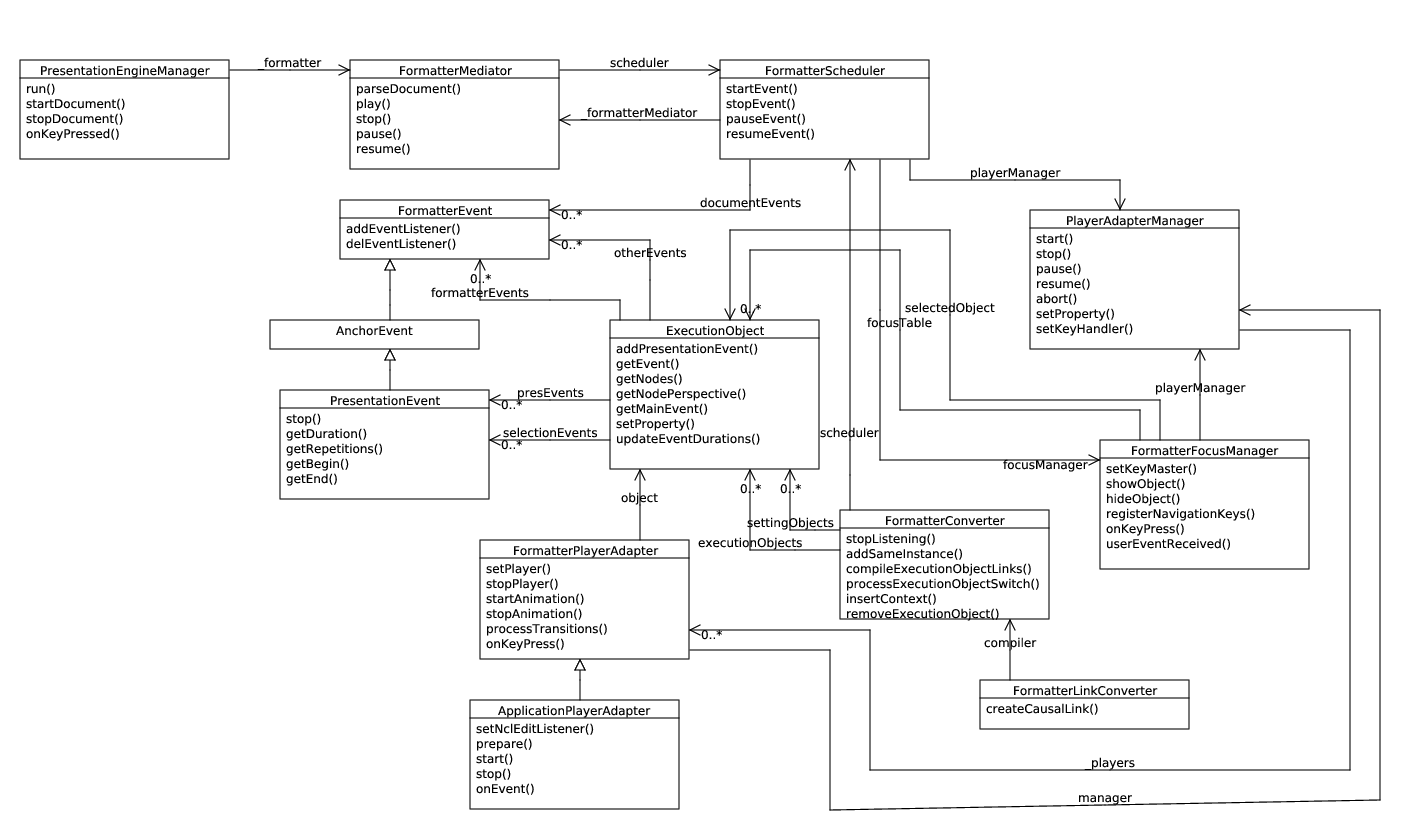
\includegraphics[scale=0.35]{resources/uml-ncl30-presenter.jpg}
	\caption{Diagrama de las principales clases de la librería \emph{ncl30-presenter}.}
\end{figure}

\FloatBarrier
